

\section{Virtual reality components}



A \acrshort{vr} system is made up of two major subsystems, the hardware and software. The hardware can be further divided into \acrshort{vr} engine and I/O devices, while the software can be divided into application software and database as illustrated in Figure \ref{fig:sys}.
The classical five components of a \acrshort{vr} system are, Software and Database, \acrshort{vr} Engine, I/O Devices, User and Task \citep{burdea2017virtual,Bamodu2013VirtualComponents}.

\begin{figure}[ht]
    \centering
    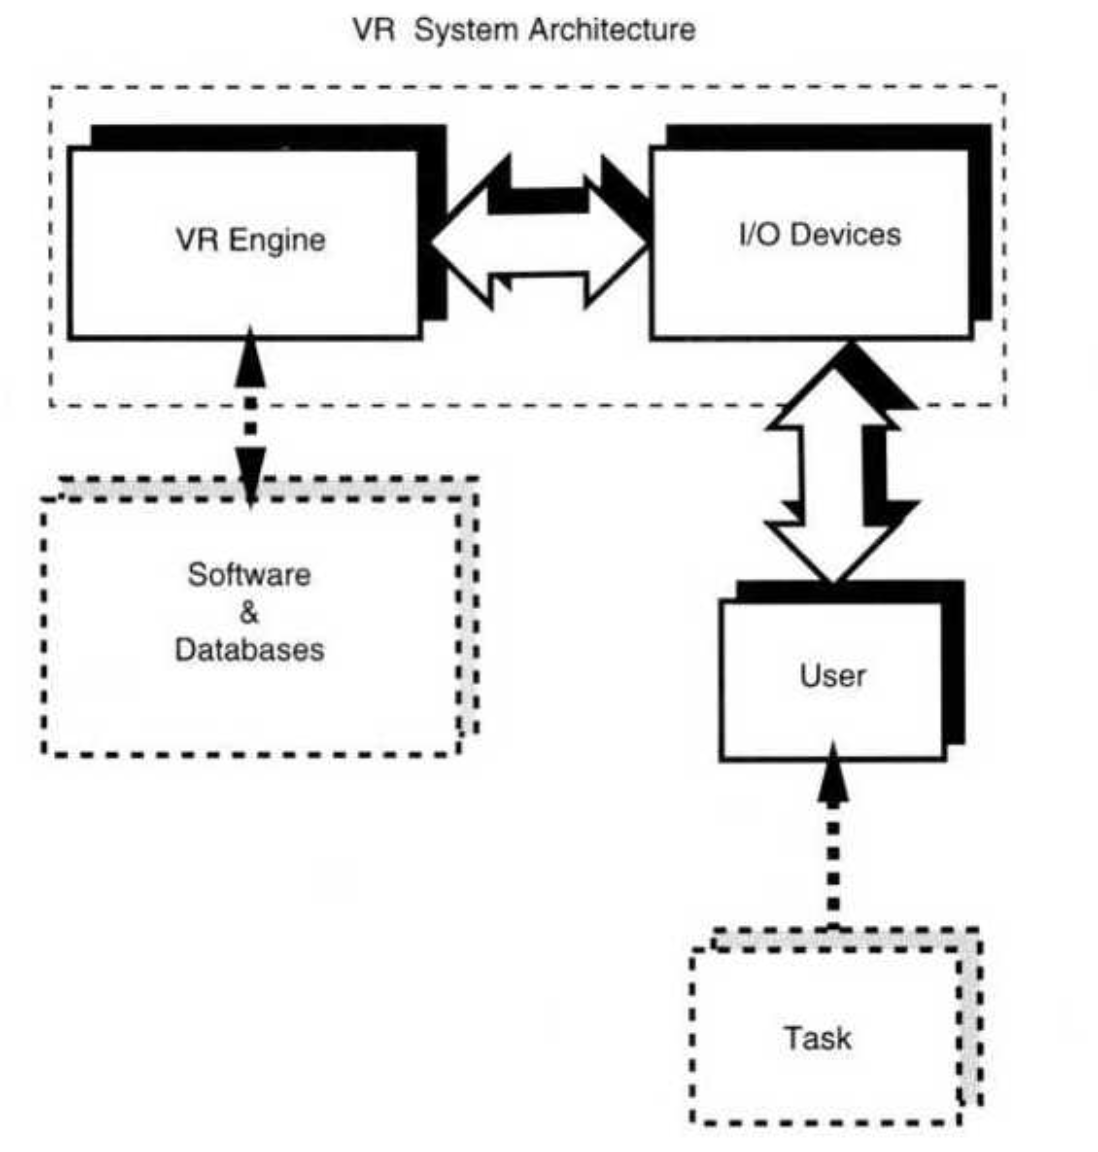
\includegraphics[width=0.50\textwidth]{images/VR.png}
    \caption{VR System Architecture - \citep{burdea2017virtual}}
    \label{fig:sys}
\end{figure}


\subsection{Software and Database}
Virtual reality system software is a colletion of tools and software for designing, developing and
maintaining virtual environments and the database where the information is stored. The tools can be classified into modeling tools and development tools.

VR Modeling Tools. There are many modeling tools available for VR designing, the most
common ones are , 3ds Max, Maya and Creator. Engineering specific applications might use software like CATIA, Pro/E, Solidworks, UG, etc. VR Development Tools. VR is a complex and integrative technology that borrows from many other technologies, such as real time 3D computer graphics, tracking technology, sound processing, and haptic technology, among others, therefore software development flexibility and real time interaction is needed.


\subsection{VR Engine}
VR Engine. In VR systems, the VR engine or computer system has to be selected according to the
requirement of the application. Graphic display and image generation are some of the most important factors and time consuming task in a VR system. The choice of the VE engine depends on the application field, user, I/O devices, level of immersion and the graphic output required, since it is responsible for calculating and generating graphical models, object rendering, lighting, mapping, texturing, simulation and display in real-time. The computer also handles the interaction with users and serves as an interface with the I/O devices. A major factor to consider when selecting the VR engine is the processing power of the computer, and the computer processing power is the amount of senses (graphical, sound, haptic, etc) that can be rendered in a particular time frame as pointed. The VR engine is required to recalculate the virtual environment approximately every 33ms and produce real time simulation of more than 24fps [4], furthermore, the associated graphic engine should be capable of producing stereoscopic vision. The VR engine could be a standard PC with more processing power and a powerful graphics accelerator or distributed computer systems interconnected through high speed communication network.


\subsection{I/O Devices}
Input Devices. The input devices are the means by which the user interacts with the virtual world. They send signals to the system about the action of the user, so as to provide appropriate reactions back to the user through the output devices in real time. They can be classified into tracking device, point input device, bio-controllers and voice device. Tracking devices sometimes referred to as position sensors, are used in tracking the position of the user [1], and they include, electromagnetic, ultrasonic, optical, mechanical and gyroscopic sensors, data gloves, neural and bio or muscular controllers [2]. Examples of point-input devices include 6DOF mouse and force or space ball. Their technology is an adaptation of the normal mouse with extended functions and capability for 3D. Voice communication is a common way of interaction among humans. So it feels natural to incorporate it into a VR system. Voice recognition or processing software can be used in accomplishing this.

Output Devices. The output devices get feedback from the VR engine and pass it on to the users through the corresponding output devices to stimulate the senses. The possible classifications of output devices based on the senses are: graphics (visual), audio (aural), haptic (contact or force), smell and taste. Of these, the first 3 are frequently used in VR systems, while smell and taste are still uncommon.
Two possible common options for the graphics are the stereo display monitor, and the HMD which provides a higher level of immersion. In the HMD, the two independent views produced are interpreted by the brain to provide a 3D view of the virtual world. Audio or sound is an important channel in VR; its importance is only surpassed by that of visual. 3D sound can be used in producing different sounds from different location to make the VR application more realistic.
Haptic is used to allow the user feel virtual objects. This can be achieved through electronic signals or mechanical devices.



\subsection{User}



\subsection{Task}



\section{Hardware and Development Environments}










\subsection{Headsets}
\textbf{Google Cardboard}: The virtual reality platform was released in
2014 by Google. The platform is intended as a low-cost system to
encourage interest and development in VR applications. It was
named for its fold-out cardboard viewer. The Google Cardboard
headsets are built out of simple, low-cost components -
cardboard. Google open-sourced the schematics and the
assembly instructions freely on their site, allowing people to
assemble Cardboard themselves from readily available parts (“Google Cardboard,” 2014). The
cardboards were the best option to be used for the project due to the easy mobility and the
low price. It is easier to travel with it through airports or checkpoints since it’s cardboard.
\subsection{Cameras}
\textbf{GoPro Fusion}: the footage quality can reach up to 5.2K spherical video
resolution. The GoPro fusion can be controlled via a mobile
application through Bluetooth or Wi-Fi. The two lenses on the two
sides are not symmetrically aligned, they are off-axis. That helps to
process the images or the footage taken from the two lenses to not
have visible stitching or overlapping in the final image. That is a
common problem in most of the VR cameras to have a big overlapping on the final image. The
data is saved on two microSD cards one for each lens, the files need to be combined to have
a final 360o video \citep{Easton2018}. The camera was used in most of the project filming material,
it has the best footage quality and a perfect stabilization in the videos.


\textbf{Samsung Gear 360}: The small and rounded shape of the camera is ideal for
handheld shooting, although it has a socket also for a tripod. A small LCD
screen helps in navigating through the camera modes. The video resolution is
4K, while the still images are somewhat soft. The smartphone app is easy to
use and clear for the user also it offers a good range of viewing options. In
general is it a small and simple camera to use (Digital Camera, 2018). The
camera used as a backup camera during the project. The quality is acceptable
for a small and very light camera.

\subsection{Development Environments}

The VR technology is moving forward and there is an increasing number of tools and platforms
available for developers (“11 Tools for VR Developers,” 2017). VR technology has found its
way into different environments like computers, smartphone, and web. This section will
mention the two tools that were used by the VR team developers to build a mobile VR
application and a VR experience over the web. Nevertheless, most browsers are still struggling
with the headset device support. Most phones can be detected with the WebVR-polyfill and
if turned sideways, it will switch the dual display mode automatically that you can use Google
Cardboard or other headsets built for smartphones (“11 Tools for VR Developers,” 2017).


\textbf{Unity 3D}: Unity is one of the most famous game engines, it has a direct VR mode to preview
the work on any Head mounted display, which can be easier and faster for designers to boost
their productivity. Most of the Head mounted displays are supported in Unity. Unity works
with C\# and JavaScript; it is easy to learn due to the huge online community. Unity can export
the work to almost any platform even WebGL (“11 Tools for VR Developers,” 2017). Unity was
the best and most powerful tool to be used during the project to develop the VR experience.
Due to the easy implementation of the VR Environment in Unity, also the variety of platforms
that it allows the developer to distribute the software on it. In addition, there is a huge
community for Unity developers on the internet, where everyone can share knowledge and
expertise.


\textbf{A-frame}: A Mozilla open-source project allow you to develop and experience WebVR without
the need of learning Three.js or WebGL directly. This web framework built on top of Three.js
and WebGL to build virtual reality experiences by using an Entity-Component ecosystem in
HTML (“11 Tools for VR Developers,” 2017). A-Frame was the first choice for developing the
experience over the web due to its functionality and easy implementation on webpages. A
variety of examples are offered on A-Frame website, so the user can take those examples and
build on them or reuse their code on a project since it is an open-source platform.


\section{Development \& Implementation}

\subsection{Software}

\subsection{User Interface}

“ In order to allow human-computer interaction it is necessary to use special interfaces designed to input a user's commands into the computer and to provide feedback from the simulation to the user” \citep{burdea2017virtual}.